\documentclass[
    ngerman,
    color=3b,
    dark_mode,
    load_common, % Loads a list of commonly used Packages
    summary,
    boxarc,
    % manual_term,
    % solution=true,
]{tuda_summary} 
% Import all Packages from Main Preamble with relative Path
% \subimport*{../../}{preamble}
% Get Labels from Main Document using the xr-hyper Package
\externaldocument{../../AuD-Zusammenfassung-2020}
% Set Graphics Path, so pictures load correctly
\graphicspath{{../../}}

\begin{document}
\section{Advanced Designs}\index{Advanced Designs}
\subsection{Dynamische Programmierung}\index{Dynamische Programmierung}
\paragraph{Anwendung}\mbox{}\\
Anwendung, wenn sich Teilprobleme überlappen:
\begin{enumerate}
    \item Wir charakterisieren die Struktur einer optimalen Lösung
    \item Wir definieren den Wert einer optimalen Lösung rekursiv
    \item Wir berechnen den Wert einer optimalen Lösung (meist bottom-up Ansatz)
    \item Wir konstruieren eine zugehörige optimale Lösung aus berechneten Daten
\end{enumerate}

\subsubsection{Stabzerlegungsproblem}\index{Stabzerlegungsproblem}

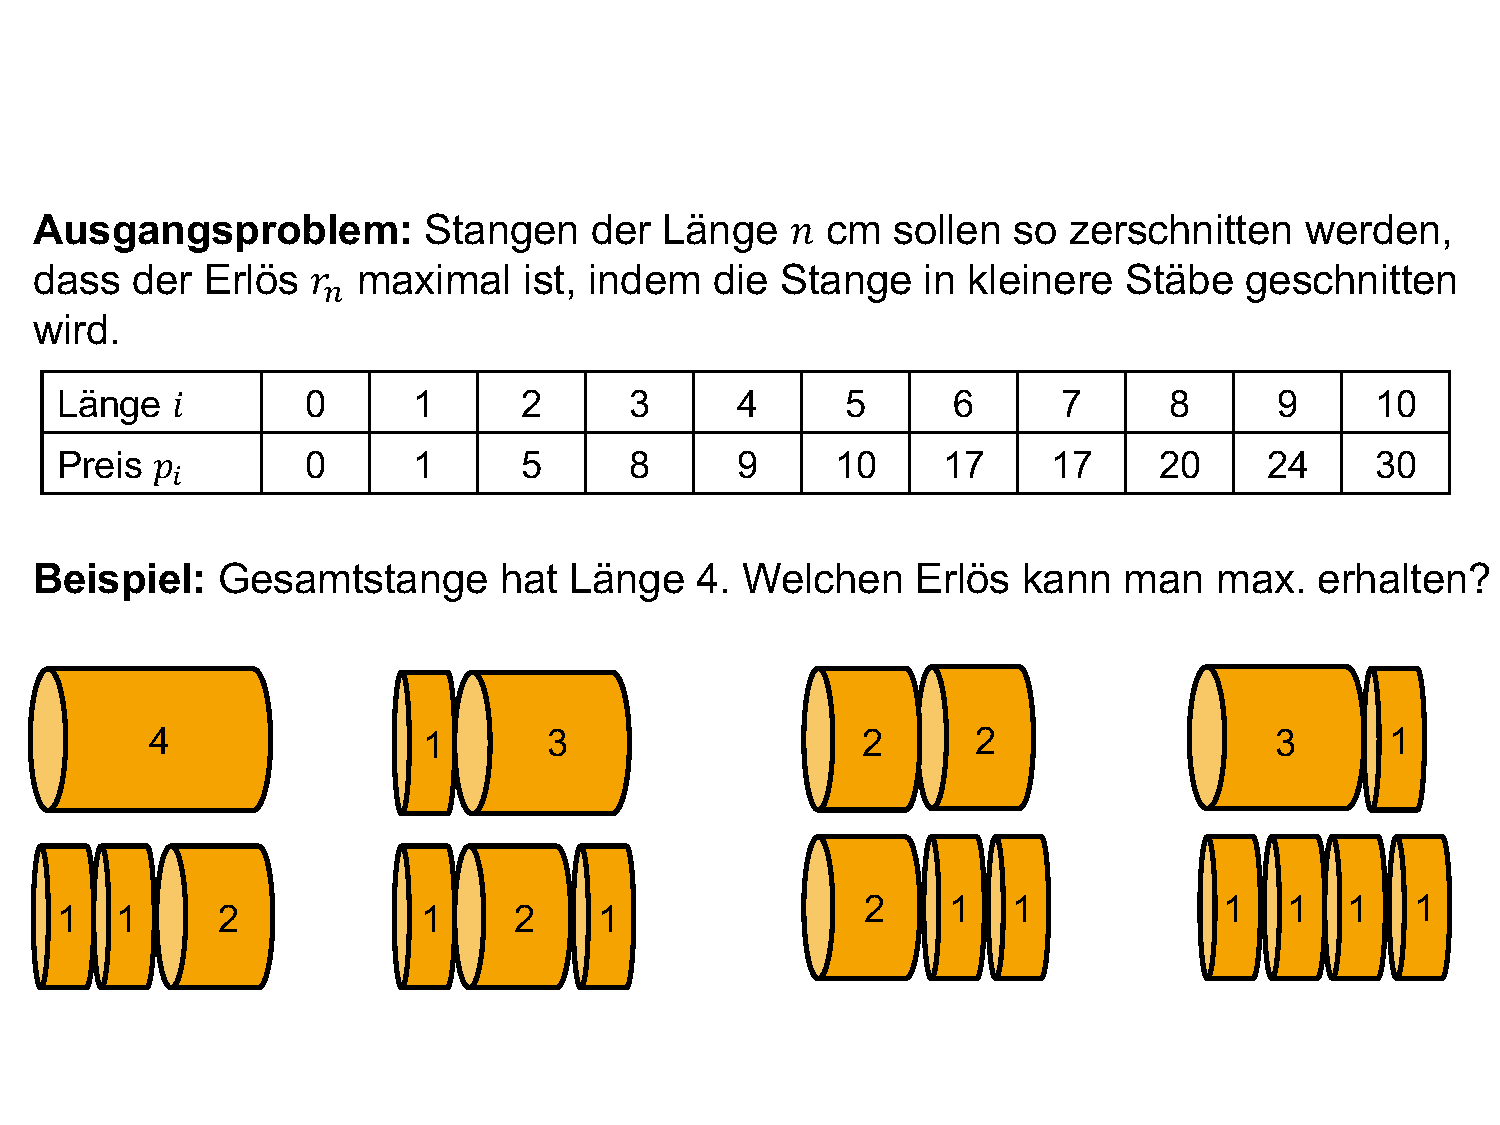
\includegraphics[width=12cm]{pictures/stabzerlegungsproblem.pdf}\\
Optimaler Erlös: zwei 2cm lange Stücke ($5+5=10$)\\
\paragraph{Aufteilung der Stange}
\begin{itemize}
    \item Stange mit Länge $n$ kann auf $2^{n-1}$ Weisen zerlegt werden
    \item Position $i$: Distanz vom linken Ende der Stange
    \item Aufteilung in $k$ Teilstäbe ($1 \leq k \leq n$)
    \item optimale Zerlegung: $n = i_1 + i_2 + ... + i_k$
    \item maximaler Erlös: $r_n = p_{i_1} + p_{i_2} + ... + p_{i_k}$
    \item z.B.: $r_4 = 10$ (siehe oben)
\end{itemize}
\clearpage
\paragraph{Rekursive Top-Down Implementierung}\mbox{}

%\begin{noindent}
\begin{codeBlock}[autogobble,escapeinside=||]{title={CUT-ROD(p,n)    // p Preis-Array, n Stangenlänge}}
    IF n == 0
        return 0;
    q = |$-\infty$|;
    FOR i = 1 TO n  // nicht Start bei 0, sonst kein Rekursionsschritt
        q = max(q, p[i] + CUT-ROD(p, n - i));
    return q;
\end{codeBlock}
%\end{noindent}
\paragraph{Stabzerlegung via Dynamischer Programmierung:}
\begin{description}[leftmargin=2cm]
    \item [Ziel]
          Mittels dynamischer Programmierung wollen wir \texttt{CUT-ROD} in einen effizienten
          Algorithmus verwandeln.
    \item [Bemerkung]
          Naiver rekursiver Ansatz ist \fatsf{ineffizient}, da dieser immer wieder diesselben
          Teilprobleme löst.
    \item [Ansatz]
          Jedes Teilproblem nur einmal lösen. Falls die Lösung eines Teilproblems nochmal benötigt
          wird, schlagen wir diese nach.
\end{description}
\begin{itemize}
    \item Reduktion von exponentieller auf polynomielle Laufzeit.
    \item Dynamische Programmierung wird zusätzlichen Speicherplatz benutzen um Laufzeit einzusparen.
\end{itemize}
\paragraph{Rekursiver Top-Down-Ansatz mit Memoisation:}\mbox{}
\begin{idea}[Rekursiver Top-Down-Ansatz mit Memoisation]\mbox{}
    Speicherung der Lösungen der Teilprobleme
\end{idea}
Laufzeit: $\Theta(n^2)$

%\begin{noindent}
\begin{codeBlock}[autogobble,escapeinside=||]{title={MEMOIZED-CUT-ROD(p, n)}}
    Let r[0...] be new array
    FOR i = 0 TO n
        r[i] = |$-\infty$|
    return MEMOIZED-CUT-ROD-AUX(p, n, r)
\end{codeBlock}
%\end{noindent}
%\begin{noindent}
\begin{codeBlock}[autogobble,escapeinside=||]{title={MEMOIZED-CUT-ROD-AUX(p, n, r)       // r new Array}}
    IF r[n] |$\geq$| 0                        // Abfrage ob vorhanden
        return r[n]
    IF n == 0
        q = 0
    ELSE
        q = |$-\infty$|
        FOR i = 1 to n
        q = max(q, p[i] + MEMOIZED-CUT-ROD-AUX(p, n - i, r))
    r[n] = q                            // Abspeichern
    return q
\end{codeBlock}
%\end{noindent}
\pagebreak
\paragraph{Bottom-Up Ansatz:}\index{Bottom-Up}
\begin{itemize}
    \item Laufzeit: $\Theta(n^2)$
    \item Sortieren der Teilprobleme nach ihrer Grö\ss e und lösen in dieser Reihenfolge
    \item Alle Teilprobleme kleiner als das momentane Problem sind bereits gelöst
\end{itemize}
\begin{minipage}[t]{.46\textwidth}\mbox{}
    %\begin{noindent}
    \begin{codeBlock}[autogobble,escapeinside=||]{title={BOTTOM-UP-CUT-ROD(p, n)}}
        Let r[0...n] be a new array
        r[0] = 0
        FOR j = 1 TO n
            q = |$-\infty$|
            FOR i = 1 TO j
                q = max(q, p[i] + r[j - i])
            r[j] = q
        return r[n]
    \end{codeBlock}
    %\end{noindent}
\end{minipage}
\begin{minipage}[t]{.54\textwidth-2.22166pt}\mbox{}
    %\begin{noindent}
    \begin{codeBlock}[autogobble,escapeinside=||]{title={EXTENDED-BOTTOM-UP-CUT-ROD(p, n)}}
        Let r[0...n] and s[0...n] be  new arrays
        r[0] = 0, s[0] = 0
        FOR j = 1 TO n
            q = |$-\infty$|
            FOR i = 1 TO j
                IF q < p[i] + r[j-i]
                    q = p[i] + r[j - i]
                    s[j] = i
            r[j] = q
        return r and s
    \end{codeBlock}
    %\end{noindent}
\end{minipage}

Teilproblemgraph ($i \rightarrow j$ bedeutet, dass Berechnung von $r_i$ den Wert $r_j$ benutzt)\\
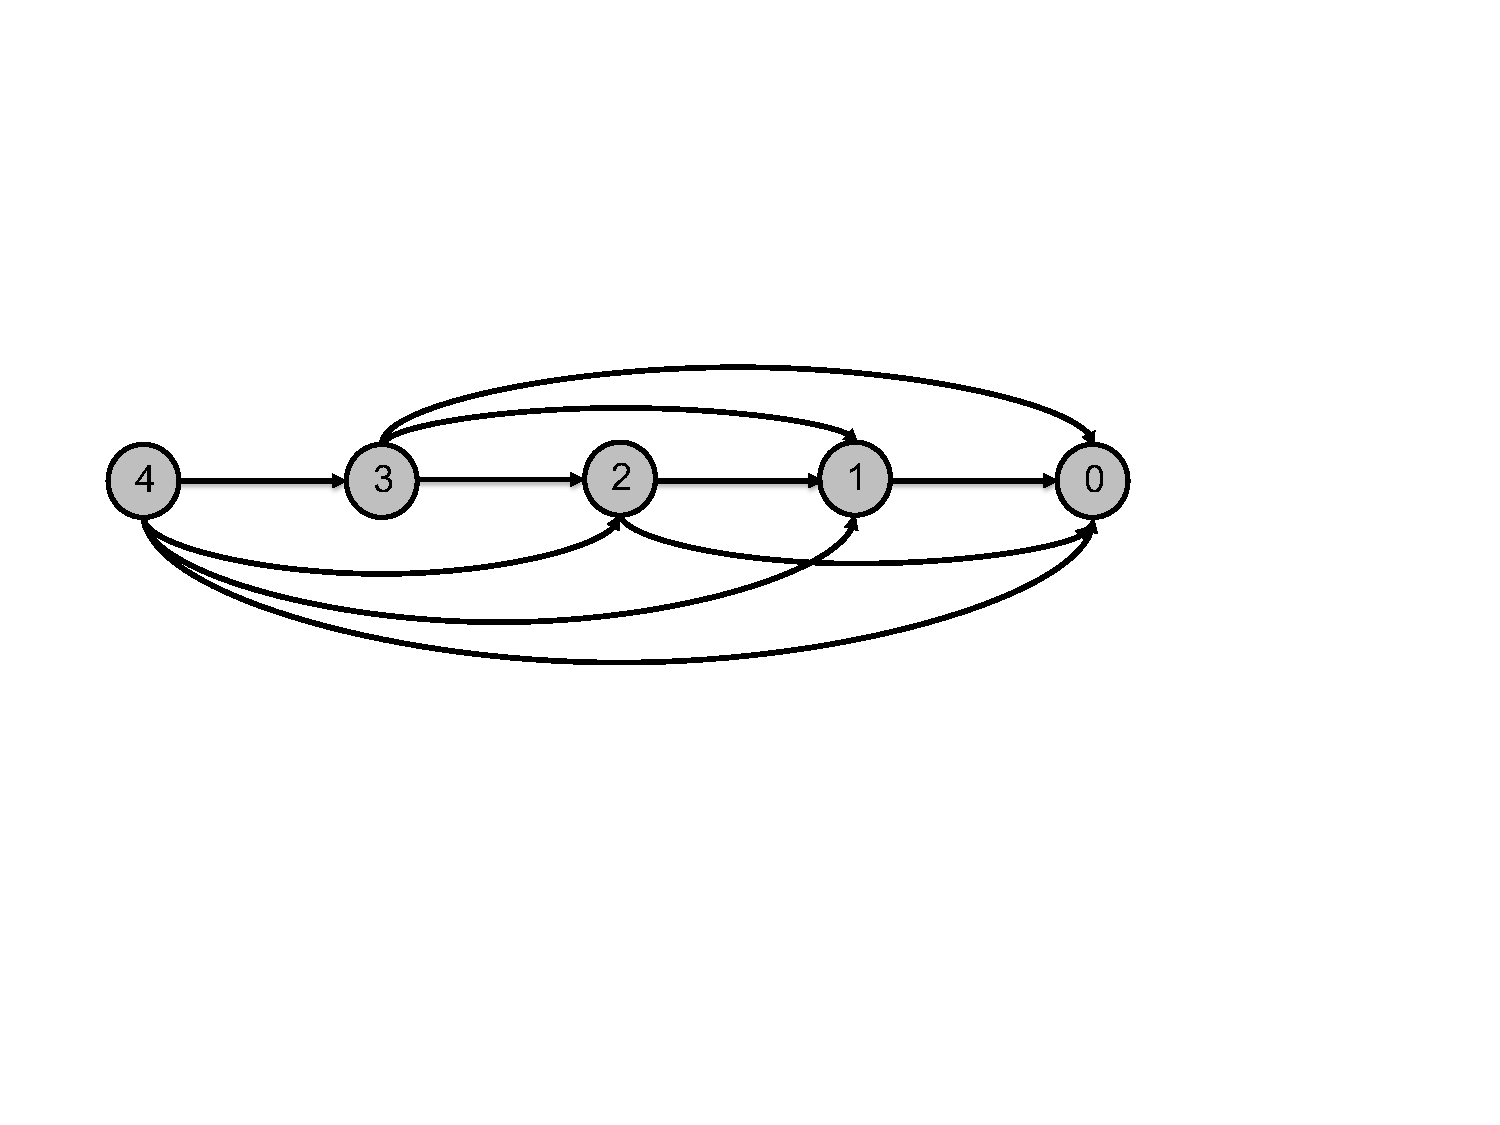
\includegraphics[width=8cm]{pictures/teilproblemgraph.pdf}


\paragraph{Fibonacci-Zahlen}\index{Fibonacci-Zahlen}
\begin{itemize}
    \item $F_1 = F_2 = 1$
    \item $F_n = F_{n-1} + F_{n-2}$
\end{itemize}
\textit{Naiver rekursiver Algorithmus:}

%\begin{noindent}
\begin{codeBlock}[autogobble,escapeinside=||]{title={FIB(n)}}
    IF n |$\leq$| 2
        f = 1;
    ELSE
        f = FIB(n-1) + FIB(n-2);
    return f;
\end{codeBlock}
%\end{noindent}
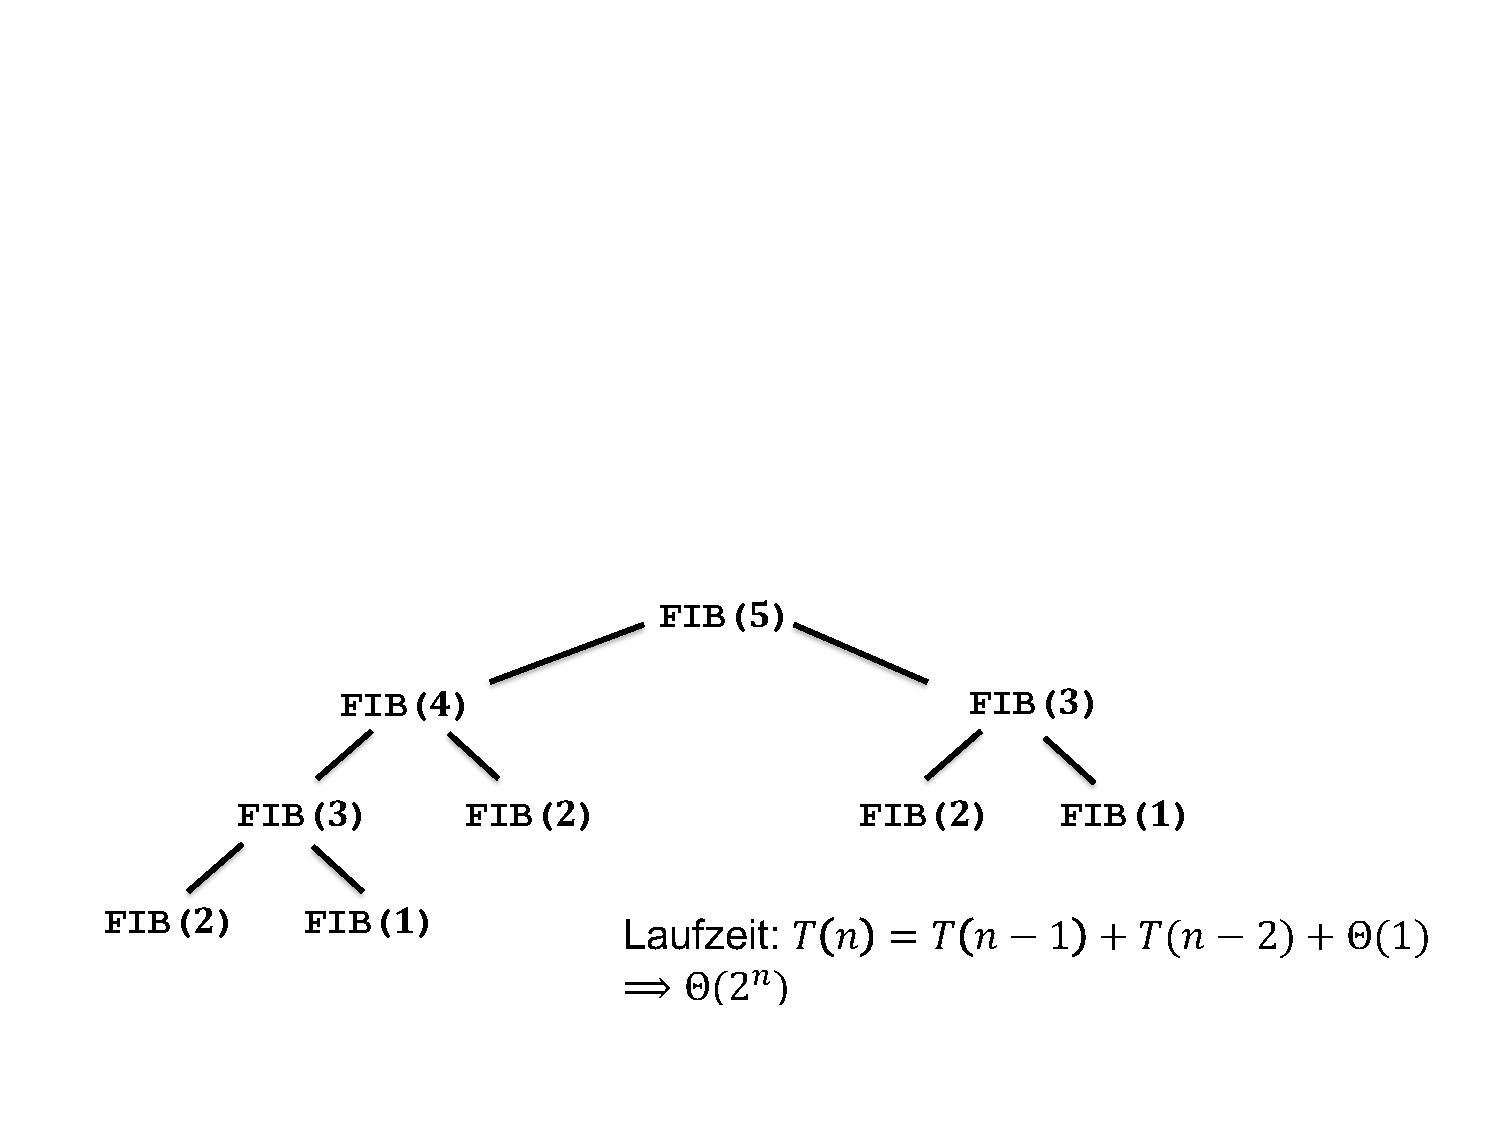
\includegraphics[width=13cm]{pictures/fibBaum.pdf}\\
Gleiche Teilprobleme werden wieder mehrmals gelöst

\clearpage
\textit{Rekursiver Algorithmus mit Memoisation:}
\begin{itemize}
    \item Wieder Abspeichern von Teilproblemen um Laufzeit einzusparen
    \item Laufzeit: $\Theta(n)$
\end{itemize}

%\begin{noindent}
\begin{codeBlock}[autogobble,escapeinside=||]{title={MEMOIZED-FIB(n)}}
    Let m[0...n-1] be a new array
    FOR i = 0 TO n - 1
        m[i] = 0
    return MEMOIZED-FIB-AUX(n, m)
\end{codeBlock}
%\end{noindent}
%\begin{noindent}
\begin{codeBlock}[autogobble,escapeinside=||]{title={MEMOIZED-FIB-AUX(n, m)}}
    IF m[n-1] != 0
        return m[n-1];      // Auslesen von gespeicherten Werten
    IF n |$\leq$| 2
        f = 1;
    ELSE
        f = MEMOIZED-FIB-AUX(n-1, m) + MEMOIZED-FIB-AUX(n-2, m);
    m[n-1] = f;
    return f;
\end{codeBlock}
%\end{noindent}

\textit{Bottom-Up Algorithmus:}

Hier wieder Berechnen aller Teilprobleme von unten beginnend

%\begin{noindent}
                            \begin{codeBlock}[autogobble,escapeinside=||]{title={BOTTOM-UP-FIB(n)}}
                            Let m[0...n] be a new array
                            FOR i = 1 TO n
                                IF i |$\leq$| 2
                                    f = 1;
                                ELSE
                                    f = m[i-1] + m[i-2];
                                m[i] = f;
                            return m[n];
                            \end{codeBlock}
                            %\end{noindent}


\clearpage
\subsection{Greedy-Algorithmus}\index{Greedy}
\begin{idea}[Greedy-Algorithmus]\mbox{}
    \begin{itemize}
        \item Trifft stets die Entscheidung, die in diesem Moment am besten erscheint
        \item Trifft \fatsf{lokale} optimale Entscheidung (evtl. nicht global die Beste)
    \end{itemize}
\end{idea}

\subsubsection{Aktivitäten-Auswahl-Problem}
\begin{definition}[Aktivitäten-Auswahl-Problem]\mbox{}
    \begin{itemize}
        \item 11 anstehende Aktivitäten $S=\{a_1,...,a_{11}\}$
        \item Startzeit $s_i$ und Endzeit $f_i$, wobei $0 \leq s_i < f_i < \infty$
        \item Aktivität $a_i$ findet im halboffenen Zeitintervall $[s_i,f_i)$ statt
        \item Zwei Aktivititäten sind kompatibel, wenn sich deren Zeitintervalle nicht überlappen
    \end{itemize}
\end{definition}

\begin{minipage}{0.6\textwidth}
    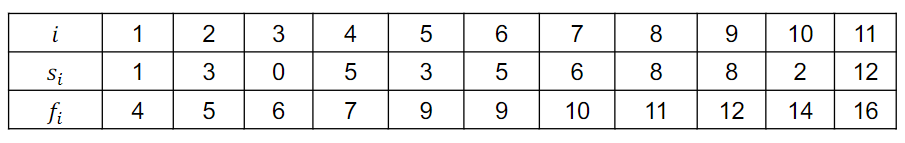
\includegraphics[width=10cm]{pictures/aktivProblem1.PNG}
\end{minipage}
\begin{minipage}{0.3\textwidth}
    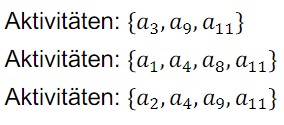
\includegraphics[width=4cm]{pictures/aktivProblem2.PNG}
\end{minipage}

\paragraph{Ansatz mittels dynamischer Programmierung}
\begin{itemize}
    \item Menge von Aktivitäten, die starten nachdem $a_i$ endet und enden, bevor $a_j$ startet \\
          $S_{ij} = \{a \in S,a = (s,f): s \geq f_i, f < s_j\}$
    \item Definiere maximale Menge $A_{ij}$ von paarweise kompatiblen Aktivitäten in $S_{ij}$. \\
          $c[i,j] = |A_{ij}|$
    \item Optimale Lösung für Menge $S_{ij}$ die Aktivitäten $a_k$ enthält: \\
          $c[i,j] = max_{a_k\in S_{ij}}\{c[i,k] + c[k,j] + 1\}$ ($0$, falls $S_{ij} = \emptyset$)
\end{itemize}

\paragraph{Greedy-Wahl}
\begin{itemize}
    \item lokal die beste Wahl
    \item Auswahl der Aktivität mit geringster Endzeit (möglichst viele freie Ressourcen)
    \item Also hier Teilprobleme, die nach $a_1$ starten
    \item $S_k = \{a_i \in S: s_i \geq f_k\}$: Menge an Aktivitäten, die starten, nachdem $a_k$ endet
    \item \textit{Optimale-Teilstruktur-Eigenschaft} \\
          Wenn $a_1$ in optimaler Lösung enthalten ist, dann besteht optimale Lösung zu ursprünglichem
          Problem aus Aktivität $a_1$ und allen Aktivitäten zur einer optimalen Lösung des
          Teilproblems $S_1$
\end{itemize}
\clearpage
\paragraph{Rekursiver Greedy-Algorithmus}\mbox{}
\begin{grayInfoBox}
    \fatsf{Voraussetzung}: Aktivitäten sind monoton steigend nach der Endzeit sortiert
\end{grayInfoBox}
Laufzeit: $\Theta(n)$

%\begin{noindent}
\begin{codeBlock}[autogobble,escapeinside=||]{title={RECURSIVE-ACTIVITY-SELECTOR(s,f,k,n)}}
    // s Anfangszeitenarray, f Endzeitenarray, 
    // k Index von Teilproblem, n Grö\ss{}e Anfangsproblem
    m = k + 1;
    WHILE m |$\leq$| n and s[m] < f[k]  // Suche nach erster Kompatibilität
        m = m + 1;
    IF m |$\leq$| n
        // Ausgabe des Elements und Berechnung weiterer Aktivitäten
        return {|$a_m$|} |$\cup$| RECURSIVE-ACTIVITY-SELECTOR(s,f,m,n)
    ELSE
        return |$\emptyset$|
\end{codeBlock}
%\end{noindent}

\paragraph{Iterativer Greedy-Algorithmus}\mbox{}
\begin{grayInfoBox}
    \fatsf{Voraussetzung}: Aktivitäten sind monoton steigend nach der Endzeit sortiert
\end{grayInfoBox}
Laufzeit: $\Theta(n)$
%\begin{noindent}
\begin{codeBlock}[autogobble,escapeinside=||]{title={GREEDY-ACTIVITY-SELECTOR(s,f)}}
    n = s.length;
    A = {|$a_1$|};
    k = 1;          // Index des zuletzt hinzugefügten Elements in A
    FOR m = 2 TO n                      
        IF s[m] |$\geq$| f[k]       // Findet zuerst endende Aktivität in Menge
            A = A |$\cup$| {|$a_m$|};   // Fügt diese hinzu, falls kompatibel
            k = m;
    return A;
\end{codeBlock}
%\end{noindent}

\clearpage
\subsection{Backtracking}\index{Backtracking}
\paragraph{Suchbaum - Baum der Möglichkeiten}\mbox{}\\
Darstellung aller für ein Problem bestehenden Möglichkeiten\\
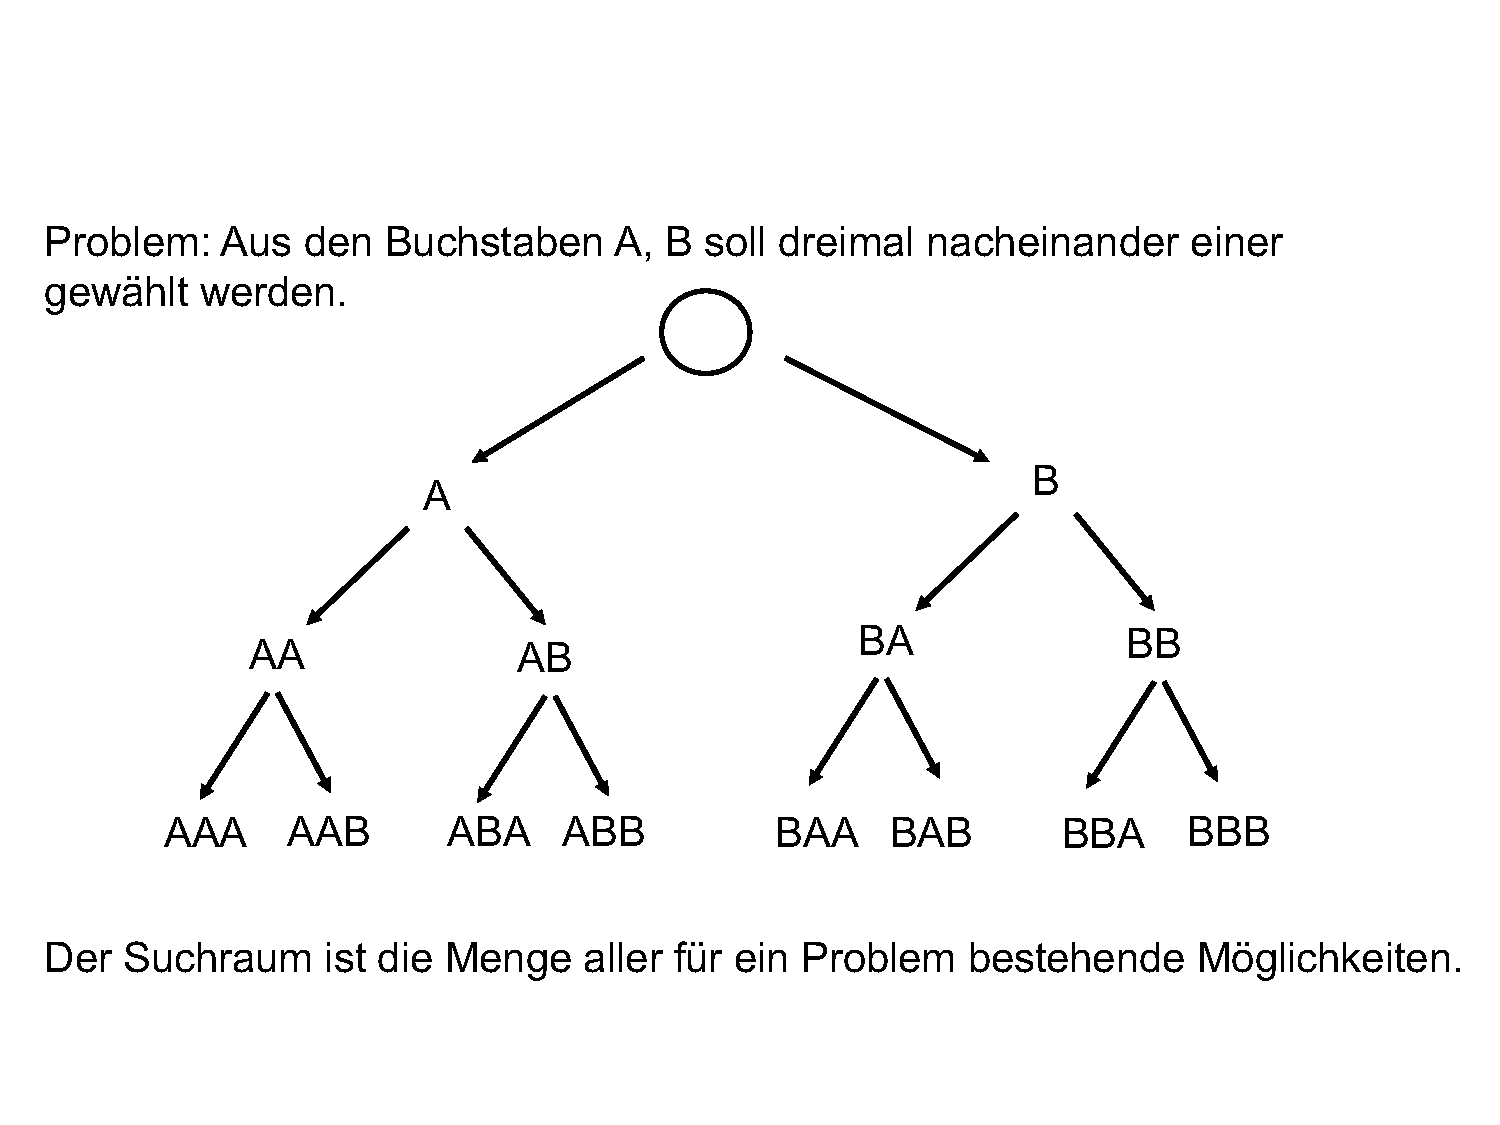
\includegraphics[width=14cm]{pictures/suchbaum.pdf}
\begin{idea}[Backtracking]\mbox{}
    \begin{itemize}
        \item Lösung finden via Trial and error
        \item Schrittweises Herantasten an die Gesamtlösung
        \item Falls Teillösung inkorrekt $\rightarrow$ Gehe einen Schritt zurück und probiere eine andere Möglichkeit
        \item Voraussetzung:
              \begin{itemize}
                  \item Lösung setzt sich aus Komponenten zusammen (Sudoku, Labyrinth,..)
                  \item Mehrere Wahlmöglichkeiten für jede Komponente
                  \item Teillösung kann auf Korrektheit getestet werden
              \end{itemize}
    \end{itemize}
\end{idea}
\paragraph{Allgemeiner Backtracking-Algorithmus}\mbox{}
%\begin{noindent}
\begin{codeBlock}[autogobble]{title={BACKTRACKING(A, s)}}
    IF alle Komponenten richtig gesetzt
        return true;
    ELSE
        WHILE auf aktueller Stufe gibt es Wahlmöglichkeiten
            wähle einen neuen Teillösungsschritt
            Teste Lösungsschritt gegen vorliegende Einschränkungen
            IF keine Einschränkung THEN
                setze die Komponente
            ELSE
                Auswahl(Komponente) rückgängig machen
            BACKTRACKING(A, s + 1)
\end{codeBlock}
%\end{noindent}

\clearpage
\paragraph{Damenproblem}\index{Damenproblem}\mbox{}\\
Auf einem Schachbrett der Grö\ss{}e $n \cdot n$ sollen $n$ Damen so positioniert werden, dass sie sich
gegenseitig nicht schlagen können. Wie viele Möglichkeiten gibt es, $n$ Damen so aufzustellen, dass keine
Damen eine andere schlägt.
\begin{minipage}{7cm}
    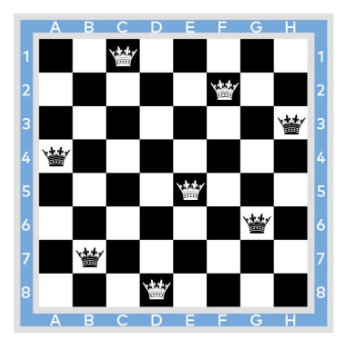
\includegraphics[width=6cm]{pictures/damenproblem.PNG}
    \captionof{figure}{Beispielhafte Darstellung des Damenproblems}
\end{minipage}
\begin{minipage}{\textwidth-7cm}
    \begin{itemize}
        \item $n=8:$ 4 Milliarden Positionierungen
        \item Optimierte Suche: In jeder Zeile/Spalte nur eine Dame
        \item Reduziert Problem auf 40.000 Positionierungen (ohne Diagonale)
    \end{itemize}
\end{minipage}
%\begin{noindent}
\begin{codeBlock}[autogobble]{title={PLACE-QUEENS(Q,r) // Q Array von Damenpositionen, r Index der ersten leeren Zeile}}
    IF r == n
        return Q;
    ELSE
        FOR j = 0 TO n - 1 // Mögliche Positionierungen
            legal = true;
            FOR i = 0 TO r - 1  // Evaluation der mgl. Bedrohungen
                IF (Q[i] == j) OR (Q[i == j + r - i]) OR (Q[i] == j - r + i)
                    legal = false;
            IF legal == true
                Q[r] = j;
                PLACE-QUEENS(Q, r + 1)
\end{codeBlock}
%\end{noindent}
\begin{figure}[h]
    \centering
    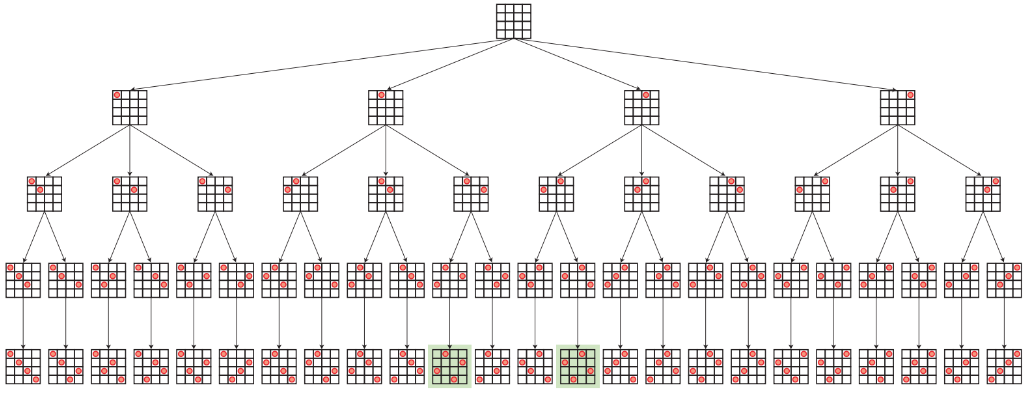
\includegraphics[width=16cm]{pictures/damenSuchbaum.PNG}
    \caption{Mögliche Pfade von Place-Queens}
\end{figure}



\pagebreak

\subsection{Metaheuristiken}\index{Metaheuristiken}
\paragraph{Optimierungsproblem}\index{Optimierungsproblem}\mbox{}\\
\begin{minipage}{10cm}
    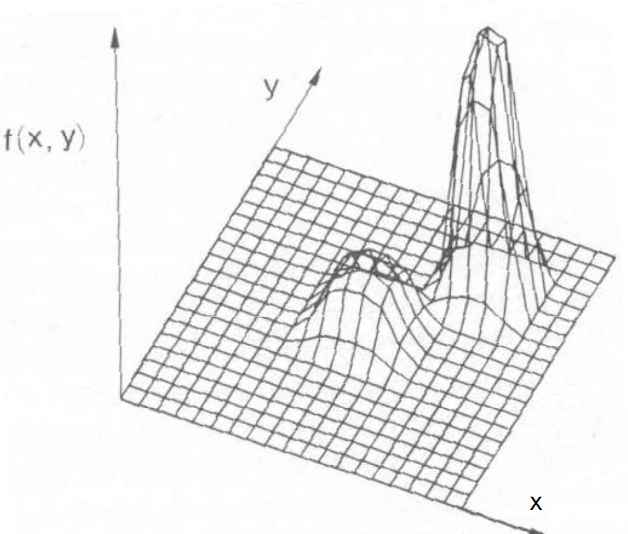
\includegraphics[width=10cm]{pictures/optimierungsproblem.PNG}
    \captionof{figure}{Beispiel Optimierungsproblem}
\end{minipage}
\begin{minipage}{\textwidth-10cm-2.22168pt}
    \begin{itemize}
        \item Lösungsstrategien:
              \begin{itemize}
                  \item Exakte Methode
                  \item Approximationsmethode
                  \item Heuristische Methode
              \end{itemize}
        \item Einschränkungen
              \begin{itemize}
                  \item Antwortzeit
                  \item Problemgrö\ss{}e
              \end{itemize}
        \item[] $\Rightarrow$ exkludieren oft exakte Methoden
    \end{itemize}
\end{minipage}


\paragraph{Heuristik}\index{Heuristik}
\begin{itemize}
    \item Technik um Suche zur Lösung zu führen
    \item Metaheuristik (Higher-Level-Strategie)
          \begin{itemize}
              \item soll z.B. Hängenbleiben bei lokalem Maxima verhindern
          \end{itemize}
    \item \textit{Leiten einer Suche}
          \begin{enumerate}
              \item Finde eine Lösung (z.B. mit Greedy-Algorithmus)
              \item Überprüfe die Qualität der Lösung
              \item Versuche eine bessere Lösung zu finden
                    \begin{itemize}
                        \item Herausfinden in welcher Richtung bessere Lösung evtl. liegt
                        \item ggf. Wiederholung dieses Prozesses
                    \end{itemize}
          \end{enumerate}
    \item \textit{Finden einer besseren Lösung}
          \begin{itemize}
              \item Modifikation der Lösung durch erlaubte Operationen
              \item Dadurch erhalten wir Nachbarschaftslösungen
              \item[] $\Rightarrow$ Suche nach besseren Lösungen in der Nachbarschaft
          \end{itemize}
\end{itemize}
\clearpage
\paragraph{Rucksackproblem}\index{Rucksackproblem}\mbox{}
\begin{grayInfoBox}
    \fatsf{Ziel:} Höchster Wert der Gegenstände im Rucksack
\end{grayInfoBox}
Beispiel:
\begin{figure}[h]
    \centering
    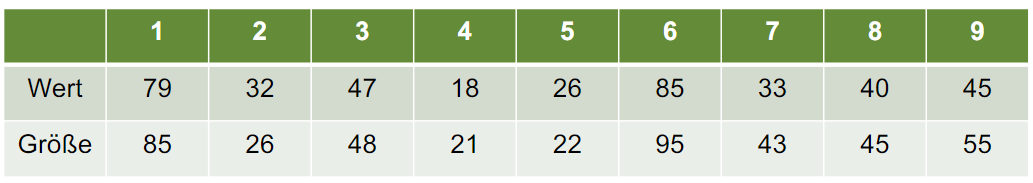
\includegraphics[width=12cm]{pictures/rucksack1.PNG}
    \caption{Beispielgegenstände für Rucksackproblem}
\end{figure}
\begin{itemize}
    \item Rucksack hat eine Kapazität von 101, 9 verschiedene Gegenstände
\end{itemize}
\begin{itemize}
    \item Beispiellösung: Gegenstand 3 + 5 (Wert 73, Grö\ss{}e 70)
    \item Nachbarschaftslösungen:
          \begin{itemize}
              \item Gegenstände 2,3 und 5: Wert 105, Grö\ss{}e 96
              \item Gegenstände 1,3 und 5: Wert 152, Grö\ss{}e 155 (Gewichtsüberschreitung problematisch)
              \item Gegenstand 3: Wert 47, Grö\ss{}e 48
          \end{itemize}
\end{itemize}
\begin{minipage}{7.2cm}
    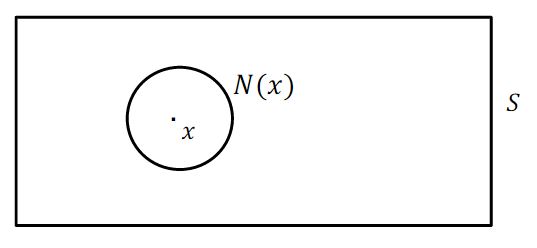
\includegraphics[width=7cm]{pictures/nachbarschaft.PNG}
\end{minipage}
\begin{minipage}{\textwidth-7.2cm-2.22168pt}
    \fatsf{Nachbarschaft:}
    \begin{itemize}
        \item Suchraum $S$ kann sehr gro\ss{} sein
        \item Einschränkung des Suchraums in der Nähe der Startlösung x
        \item Distanzfunktion $d: S x S \rightarrow \mathbb{R}$
        \item Nachbarschaft: $N(x) = \{y \in S: d(x,y) \leq \epsilon\}$
    \end{itemize}
\end{minipage}
\clearpage
\paragraph{Zufällige Suche}\mbox{}
\begin{idea}[Zufällige Suche]\mbox{}
    \begin{itemize}
        \item Suche nach globalem Optimum
        \item Anwenden der Technik auf \fatsf{aktuelle} Lösung im Suchraum
        \item Wahl einer neuen zufälligen Lösung in jeder Iteration
        \item Falls die neue Lösung besseren Wert liefert $\Rightarrow$ als neue \fatsf{aktuelle} Lösung setzen
        \item Terminierung, falls keine weiteren Verbesserungen auffindbar oder Zeit vorbei
    \end{itemize}
\end{idea}
\textit{Code:}

%\begin{noindent}
\begin{codeBlock}[autogobble]{title={RANDOM-SEARCH}}
best <- irgendeine initiale zufällige Lösung
REPEAT
    S <- zufällige Lösung // von "best" unabhängig
    IF (Quality(S) > Quality(best)) THEN
        best <- S
UNTIL best ist die ideale Lösung oder Zeit ist vorbei
return best
\end{codeBlock}
%\end{noindent}
\begin{description}[leftmargin=2cm,itemsep=.8em]
    \item[Nachteile] \begin{itemize}
              \item Potentiell lange Laufzeit
              \item Laufzeit abhängig von der initialien Konfiguration
          \end{itemize}
    \item[Vorteile] \begin{itemize}
              \item Algorithmus \fatsf{kann} beim globalen Optimum terminieren
          \end{itemize}
\end{description}

\clearpage
\paragraph{Bergsteigeralgorithmus}\index{Bergsteigeralgorithmus}\mbox{}
\begin{idea}[Bergsteigeralgorithmus]\mbox{}
    \begin{itemize}
        \item Nutzung einer iterativen Verbesserungstechnik
        \item Anwenden der Technik auf \fatsf{aktuelle} Lösung im Suchraum
        \item Auswahl einer neuen Lösung aus Nachbarschaft in jeder Iteration
        \item Falls diese besseren Wert liefert, überschreiben der \fatsf{aktuellen} Lösung
        \item Falls nicht, Wahl einer anderen Lösung aus Nachbarschaft
        \item Terminierung, falls keine weiteren Verbesserungen auffindbar oder Zeit vorbei
    \end{itemize}
\end{idea}
\textit{Code}

%\begin{noindent}
\begin{codeBlock}[autogobble,fontsize=\small]{title={HILL-CLIMBER}}
    T <- Distribution von möglichen Zeitintervallen
    S <- irgendeine initiale zufällige Lösung
    best <- S
    REPEAT
        time <- zufälliger Zeitpunkt in der Zukunft aus T
        REPEAT
            wähle R aus der Nachbarschaft von S
            IF Quality(R) > Quality(S) THEN
                S <- R
        UNTIL S ist ideale Lösung oder time ist erreicht oder totale Zeit erreicht
        IF Quality(S) > Quality(best) THEN
            best <- S
        S <- irgendeine zufällige Lösung
    UNTIL best ist die ideale Lösung oder totale Zeit erreicht
    return best
\end{codeBlock}
%\end{noindent}
\begin{description}[leftmargin=2cm,itemsep=1em]
    \item[Nachteile] \begin{itemize}
              \item Algorithmus terminiert in der Regel bei lokalem Optimum
              \item Keine Auskunft, inwiefern sich lokale Lösung von Globaler unterscheidet
              \item Optimum abhängig von Initialkonfiguration
          \end{itemize}
    \item[Vorteile] \begin{itemize}
              \item Einfach anzuwenden
          \end{itemize}
\end{description}

\clearpage
\paragraph{Iterative lokale Suche}\mbox{}
\begin{idea}[Iterative lokale Suche]\mbox{}
    \begin{itemize}
        \item Suche nach anderen lokalen Optima bei Fund eines lokalen Optimas
        \item Lösungen nur in der Nähe der \string"Homebase\string"
        \item Entscheidung, ob neue oder alte Lösung
        \item Bergsteigeralgo zu Beginn, danach aber gro\ss{}en Sprung um anderes Optimum zu finden
    \end{itemize}
\end{idea}

\textit{Code}
%\begin{noindent}
\begin{codeBlock}[autogobble,fontsize=\small]{title={ITERATIVE-LOCAL-SEARCH}}
    T <- Distribution von möglichen Zeitintervallen
    S <- irgendeine initiale zufällige Lösung
    H <- S      // Wahl des Homebasepunktes
    best <- S
    REPEAT
        time <- zufälliger Zeitpunkt in der Zukunft aus T
        REPEAT
            wähle R aus der Nachbarschaft von S
            IF Quality(R) > Quality(S) THEN
                S <- R
        UNTIL S ist ideale Lösung oder time ist erreicht oder totale Zeit erreicht
        IF Quality(S) > Quality(best) THEN
            best <- S
        H <- NewHomeBase(H,S)
        S <- Perturb(H)
    UNTIL best ist die ideale Lösung oder totale Zeit erreicht
    return best
\end{codeBlock}
%\end{noindent}
\begin{description}[leftmargin=3cm,itemsep=1em]
    \item[Perturb] \begin{itemize}
              \item ausreichend weiter Sprung (au\ss{}erhalb der Nachbarschaft)
              \item Aber nicht soweit, dass es eine zufällige Wahl ist
          \end{itemize}
    \item[NewHomeBase] \begin{itemize}
              \item wählt die neue Startlösung aus
              \item Annahme neuer Lösungen nur, wenn die Qualität besser ist
          \end{itemize}
\end{description}

\clearpage

\paragraph{Simulated Annealing}\index{Simulated Annealing}\mbox{}
\begin{idea}[Simulated Annealing]\mbox{}
    \begin{itemize}
        \item Wenn neue Lösung besser, dann wird diese immer gewählt
        \item Wenn neue Lösung schlechter, wird diese mit gewisser Wahrscheinlichkeit gewählt: \\
              $Pr(R,S,t) = e \frac{Quality(R)-Quality(S)}{t}$
        \item Der Bruch ist negativ, da $R$ schlechter ist als $S$
    \end{itemize}
\end{idea}
%\begin{noindent}
\begin{codeBlock}[autogobble,escapeinside=||]{title={SIMULATED-ANNEALING}}
    t <- Temperatur, initial eine hohe Zahl
    S <- irgendeine initiale zufällige Lösung
    best <- S
    REPEAT
        wähle R aus der Nachbarschaft von S
        IF Quality(R) > Quality(S) oder zufälliges
                    |$ Z \in [0,1] < e \frac{Quality(R)-Quality(S)}{t}$| THEN
                S <- R
        dekrementiere t
        IF Quality(S) > Quality(best) THEN
            best <- S 
    UNTIL best ist die ideale Lösung oder Temperatur |$\leq$| 0
    return best
\end{codeBlock}
%\end{noindent}
\vspace{-1em}
\paragraph{Tabu-Search}\mbox{}
\begin{idea}[Tabu-Search]\mbox{}
    \begin{itemize}
        \item Speichert alle bisherigen Lösungen und Liste und nimmt diese nicht nochmal
        \item Kann sich jedoch wieder von der optimalen Lösung entfernen
        \item Tabu List hat maximale Grö\ss e, falls voll, werden älteste Lösungen gelöscht
    \end{itemize}
\end{idea}
%\begin{noindent}
\begin{codeBlock}[autogobble,escapeinside=||,fontsize=\footnotesize]{title={TABU-SEARCH}}
    l <- maximale Grö|\ss{}|e der Tabu List
    n <- Anzahl der zu betrachtenden Nachbarschaftslösungen
    S <- irgendeine initiale zufällige Lösung
    best <- S
    L <- { } Tabu List der Länge l
    Füge S in L ein
    REPEAT
        IF Length(L) > l THEN
            Entferne ältestes Element aus L
        wähle R aus Nachbarschaft von S
        FOR n - 1 mal DO
            Wähle W aus Nachbarschaft von S
            IF W |$\notin$| L und (Quality(W) > Quality(R)) oder R |$\in$| L) THEN
                R <- W
        IF R |$\notin$| L THEN
            S <- R
            Füge R in L ein
        IF Quality(S) > Quality(best) THEN
            best <- S
    UNTIL best ist die ideale Lösung oder totale Zeit erreicht
    return best
\end{codeBlock}
%\end{noindent}


\clearpage

\paragraph{Populationsbasierte Methode}
\begin{itemize}
    \item Bisher: Immer nur Betrachtung einer einzigen Lösung
    \item Hier: Betrachtung einer Stichprobe von möglichen Lösungen
    \item Bei der Bewertung der Qualität spielt die Stichprobe die Hauptrolle
    \item z.B. Evolutionärer Algorithmus
\end{itemize}

\paragraph{Evolutionärer Algorithmus}\mbox{}
\begin{idea}[Evolutionärer Algorithmus]\mbox{}
    \begin{itemize}
        \item Algorithmus aus der Klasse der Evolutionary Computation
        \item \textit{generational Algorithmus:} Aktualisierung der gesamten Stichprobe pro Iteration
        \item \textit{steady-state Algorithmus:} Aktualisierung einzelner Kandidaten der Probe pro Iteration
        \item \textit{Resampling-Technik:} Generierung neuer Strichproben basierend auf vorherigen Resultaten
    \end{itemize}
\end{idea}
\textit{Abstrakter Code (Allgemeiner Breed und Join):}
%\begin{noindent}
\begin{codeBlock}[autogobble,escapeinside=||]{title={ABSTRACT-EVOLUTIONARY-ALGORITHM}}
    P <- generiere initiale Population
    best <- |$\boxdot$| // leere Menge
    REPEAT
        AssesFitness(P)
        FOR jedes individuelle |$P_i \in P$| DO
            IF best = |$\boxdot$| oder Fitness(|$P_i$|) > Fitness(best) THEN
                best <- |$P_i$|
        P <- Join(P, Breed(P))
    UNTIL best ist die ideale Lösung oder totale Zeit erreicht
    return best
\end{codeBlock}
%\end{noindent}
\begin{description}[leftmargin=2cm]
    \item [Breed] Erstellung neuer Stichprobe mithilfe Fitnessinformation
    \item [Join] Fügt neue Population der Menge hinzu
\end{description}

\textit{Initialisierung der Population}
\begin{itemize}
    \item Initialisierung durch zufälliges Wählen der Elemente
    \item Beeinflussung der Zufälligkeit bei Vorteilen möglich
    \item Diversität der Population (alle Elemente in Population einzigartig)
    \item Falls neue zufällige Wahl eines Individuums
          \begin{itemize}
              \item Entweder Vergleich mit allen bisherigen Individuen ($O(n^2)$)
              \item Oder besser: Nutzen eines Hashtables zur Überprüfung auf Einzigartigkeit ($O(n)$)
          \end{itemize}
\end{itemize}
\clearpage
\begin{idea}[Evolutionsstrategie]\mbox{}
    \begin{itemize}
        \item Generiere Population zufällig
        \item Beurteile Qualität jedes Individuums
        \item Lösche alle bis auf die $\mu$ besten Individuen
        \item Generie $\frac{\lambda}{\mu}$-viele Nachfahren pro bestes Individuum
        \item Join Funktion: Die Nachfahren ersetzen die Individuen
    \end{itemize}
\end{idea}

\textit{Algorithmus der Evolutionsstrategie}

%\begin{noindent}
\begin{codeBlock}[autogobble,escapeinside=||]{title={($\mu, \lambda$)-EVOLUTION-STRATEGY}}
    |$\mu$| <- Anzahl der Eltern (initiale Lösung)
    |$\lambda$| <- Anzahl der Kinder
    P <- {}
    FOR |$\lambda$|-oft DO
        P <- {neues zufälliges Individuum}
    best <- |$\boxdot$|
    REPEAT
        FOR jedes individuelle |$P_i \in P$| DO
            AssesFitness(|$P_i$|)
            IF best = |$\boxdot$| oder Fitness(|$P_i$|) > Fitness(best) THEN
                best <- |$P_i$|
        Q <- die |$\mu$| Individueen deren Fitness() am Grö|\ss{}|ten ist
        P <- {}
        FOR jedes Element |$Q_j \in Q$| DO
            FOR |$\frac{\lambda}{\mu}$|-oft DO
                P <- P |$\cup$| {MUTATE(|$Q_j$|)}
    UNTIL best ist die ideale Lösung oder totale Zeit erreicht
    return best
\end{codeBlock}
%\end{noindent}

\clearpage

\subsection{Amortisierte Analyse}\index{Amortisierte Analyse}
\paragraph{Kosten von Operationen}
\begin{itemize}
    \item Bisher: Betrachtung von Algorithmen, die Folge von Operationen auf Datenstrukturen ausführen
    \item Abschätzung der Kosten von $n$ Operationen im Worst-Case
    \item Dies liefert die obere Schranke für die Gesamtkosten der Operationenfolge
    \item Nun: \fatsf{Amortisierte Analyse}: Genauere Abschätzung des Worst Case
    \item Voraussetzung: Nicht alle Operationen in der Operationenfolge gleich teuer
    \item z.B. eventuell abhängig vom aktuellen Zustand der Datenstruktur
    \item Amortisierte Analyse garantiert die mittlere Performanz jeder Operation im Worst-Case
\end{itemize}

\paragraph{Beispiel Binärzähler}
\begin{description}[leftmargin=6cm,itemsep=.8em]
    \item [Eigenschaften]
          \begin{itemize}
              \item $k$-Bit Binärzähler hier als Array
              \item Codierung der Zahl als $x=\sum^{k-1}_{i=0}2^i b_i$
              \item Initialer Array für $x = 0$:
              \item[]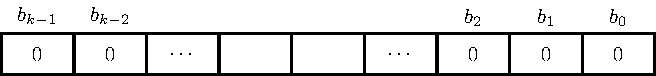
\includegraphics[width=9cm,trim={0 .8cm 0 .6cm},clip]{pictures/bitzähler.png}
          \end{itemize}
    \item [Inkrementieren eines Binärzählers]
          \begin{itemize}
              \item Erhöhe $x$ um 1
              \item Beispiel: $x=3$
              \item \texttt{INCREMENT} kostet 3, da sich drei Bitpositionen ändern
              \item[] 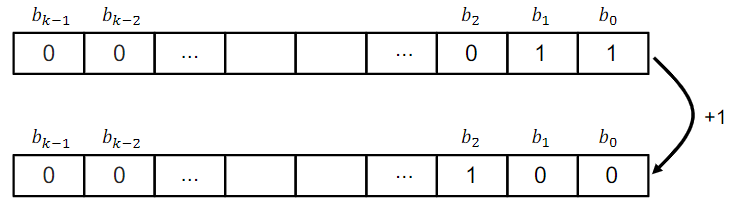
\includegraphics[width=9cm]{pictures/increment.PNG}
          \end{itemize}
          \vspace*{-.2cm}
    \item [Teuerste INCREMENT-Operation]
          \begin{itemize}
              \item \texttt{INCREMENT} flippt $k-1$ Bits von 1 zu 0 und $1$ Bit von 0 auf 1
              \item Kosten nicht konstant, stark abhängig von Datenstruktur
              \item[] 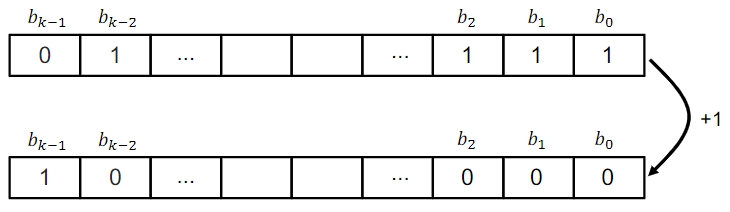
\includegraphics[width=9cm]{pictures/incrementEXP.PNG}
          \end{itemize}
    \item [Traditionelle Worst-Case Analyse]
          \begin{itemize}
              \item Worst-Case Kosten von $n$ \texttt{INCREMENT}-Operationen auf $k$-Bit Binärzähler
              \item Anfangswert $x = 0$
              \item Schlimmster Kostenfall: $INCREMENT$-Operation hat $k$ Bitflips
              \item $n$-mal inkrementieren sorgt für Kosten: $T(n) \leq n \cdot k \in O(kn)$
          \end{itemize}
\end{description}

\clearpage

\paragraph{Aggregat Methode - Beispiel Binärzähler}\mbox{}\vspace{1em}\\
\textit{Eigenschaften:}
\begin{itemize}
    \item Methode für Amortisierte Analyse
    \item Sequenz von $n$-Operationen kostet Zeit $T(n)$
    \item Durchschnittliche Kosten pro Operation $\frac{T(n)}{n}$
    \item Ziel: $T(n)$ genau berechnen, \fatsf{ohne} jedes Mal Worst-Case anzunehmen
    \item Ansatz: Aufsummation der \fatsf{tatsächlich} anfallenden Kosten aller Operationen
\end{itemize}
\textit{Durchführung:}\\

\begin{minipage}{0.5\textwidth}
    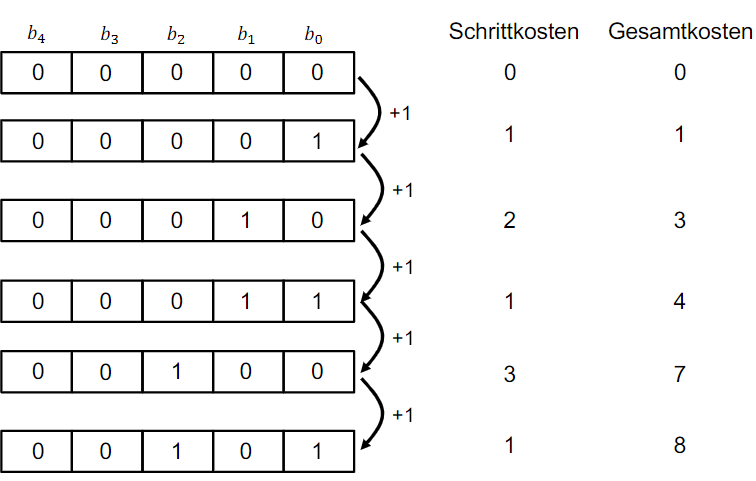
\includegraphics[width=\textwidth]{pictures/aggregat1.PNG}
\end{minipage}
\begin{minipage}{0.5\textwidth-2.22168pt}
    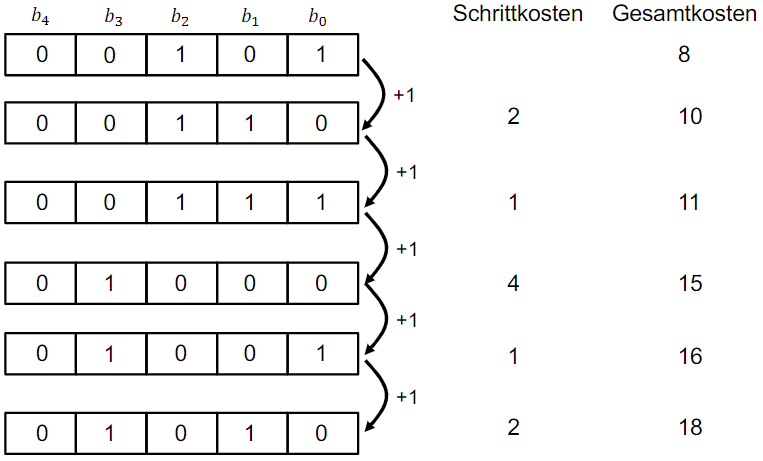
\includegraphics[width=\textwidth]{pictures/aggregat2.PNG}
\end{minipage}
\vspace{1em}\\
\begin{minipage}{0.5\textwidth}
    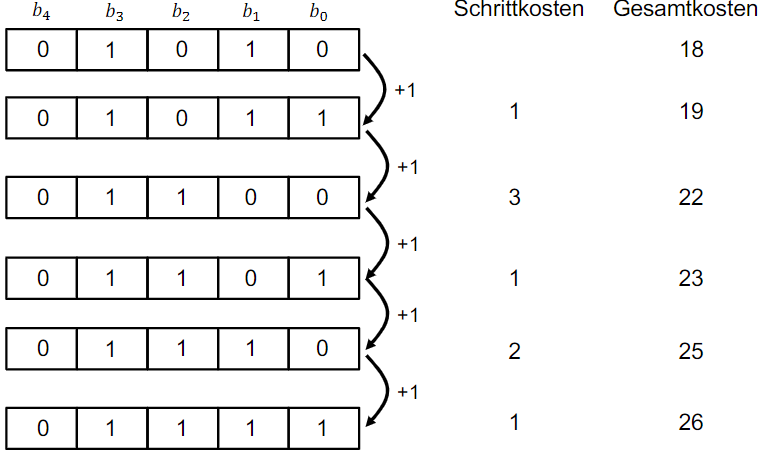
\includegraphics[width=\textwidth]{pictures/aggregat3.PNG}
\end{minipage}
\begin{minipage}{0.5\textwidth-2.22168pt}
    \begin{itemize}
        \item Bisher noch kein Worst-Case
        \item Nächste Operation hätte max. Kosten
        \item Jede 2. Operation minimale Kosten
        \item In jeder Operation ändert sich $b_0$
        \item In jeder 2. ändert sich $b_1$ etc
    \end{itemize}
\end{minipage}
\vspace{1em}\\
\textit{Genauere Kostenanalyse:}
\begin{itemize}
    \item Nun in der Lage $T(n)$ genau auszurechnen
    \item Bei $n$ Operationen ändert sich das Bit $b_i$ genau $\left \lfloor \frac{n}{2^i} \right \rfloor$-mal
    \item Bits $b_i$ mit $i > log_2~n$ ändern sich nie
    \item Über alle $k$ Bits aufsummieren liefert:
    \item[] $T(n)= \sum^{k-1}_{i=0} \left \lfloor \frac{n}{2^i} \right \rfloor = n \sum^{k-1}_{i=0} \frac{1}{2^i}
              < n \sum^{\infty}_{i=0} \frac{1}{2^i} \leq 2n \in O(n)$
    \item Obere Schranke: $T(n) \leq 2n$
    \item Kosten jeder \texttt{INCREMENT}-Operation im Durchschnitt: $\frac{2n}{n} = 2 \in O(1)$

\end{itemize}

\pagebreak

\paragraph{Account Methode - Beispiel Binärzähler}\mbox{}\vspace{1em}\\
\textit{Eigenschaften:}
          \begin{itemize}
              \item Besteuerung einiger Operationen, so dass sie Kosten anderer Operationen mittragen
              \item Zuweisung von höherern Kosten (Amortisierte Kosten), als ihre tatsächlichen Kosten sind
              \item \fatsf{Guthaben}: Differenz zwischen amortisierten und tatsächlichen Kosten
              \item Nutzung dieses Guthabens für Operationen bei denen amortisiert < tatsächlich gilt
              \item Guthaben darf nicht negativ werden:
              \item[] Summe amortisierte Kosten > Summe tatsächliche Kosten
          \end{itemize}

\textit{Wahl der Amortisierten Kosten - Binärzähler:}
          \begin{itemize}
              \item Setzen eines Bits von 0 $\rightarrow$ 1 zahlt 2 Einheiten ein / Bezeichnung $f_i$
              \item Setzen eines Bits von 1 $\rightarrow$ 0 zahlt 0 Einheiten ein / Bezeichnung $e_i$
              \item Tatsächliche Kosten $t_i$: Anzahl der Bitflips bei der $i-ten$ \texttt{INCREMENT}-Operation
              \item[] $t_i = e_i + f_i$
              \item Amortisierte Kosten betragen: $a_i = 0 \cdot e_i + 2 \cdot f_i$
          \end{itemize}

\textit{Kostenbeispiel:}
          \begin{itemize}
              \item Jede Bitflip Operation kostet zusätzlich 1 Einheit
              \item Setzen Bit 0 $\rightarrow$ 1: Zahlt 2 ein, kostet aber 1 $\rightarrow$ +1 Guthaben
              \item Setzen Bit 1 $\rightarrow$ 0: Zahlt 0 ein, kostet aber 1 $\rightarrow$ -1 Guthaben
              \item[] 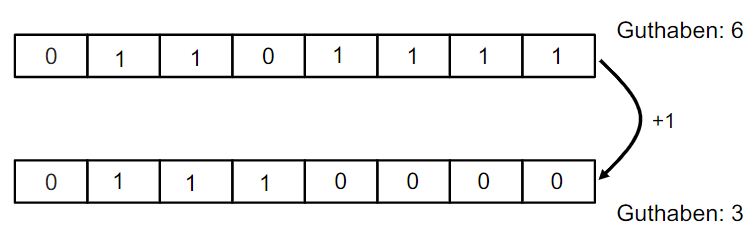
\includegraphics[width=12cm]{pictures/guthaben.PNG}
          \end{itemize}

\textit{Obere Schranken der Kosten:}
          \begin{itemize}
              \item Guthaben auf dem Konto entspricht der Anzahl der auf 1 gesetzten Bits
              \item Kosten: $T(n) \sum^n_{i=1} t_i \leq v\sum^n_{i=1} a_i$, für ein konstantes $v$
              \item Nun Abschätzung dieser Formel zum Erhalten einer oberen Schranke
              \item Beobachtung: Bei jeder \texttt{INCREMENT} höchstens ein neues Bit von 0 auf 1
              \item Für alle $i$ gilt damit $f_i \leq 1$
              \item Amortisierte Kosten jeder Operation höchstens $2 \cdot f_i \leq 2$
              \item Insgesamt: $T(n) = \sum^n_{i=1} t_i \leq \sum^n_{i=1} a_i \leq 2n \in O(n)$
          \end{itemize}

\pagebreak

\paragraph{Potential-Methode - Beispiel Binärzähler}\mbox{}\vspace{1em}\\

\textit{Eigenschaften:}
\begin{itemize}
    \item Betrachtung welchen Einfluss die Operationen auf die Datenstruktur haben
    \item Potentialfunktion $\phi(i)$: Hängt vom aktuellen Zustand der Datenstruktur nach $i$-ter Operation ab
    \item Ausgangspotential sollte vor jeglicher Operation nicht negativ sein: $\phi(0) \geq 0$
\end{itemize}

\textit{Amortisierte Kosten:}
\begin{itemize}
    \item Amortisierte Kosten der $i$-ten Operation: (Summe tatsächliche Kosten + Potentialänderung)
    \item[] $a_i = t_i + \phi(i) - \phi(i-1)$
    \item Summe der amortisierten Kosten:
    \item[] $\sum^n_{i=1} a_i = \sum^n_{i=1} (t_i + \phi(i) - \phi(i - 1)) = \sum^n_{i=1} t_i + \phi(n) - \phi(0)$
    \item Wenn für jedes $i$ gilt $\phi(i) \geq \phi(0)$:
    \item[] Summe der amor. Kosten ist gültige obere Schranke an Summe der tatsächlichen Kosten
\end{itemize}

\textit{Potential-Methode anhand des Binärzählers:}
\begin{itemize}
    \item $\phi(i)$: Anzahl der 1-en im Array nach $i$-ter \texttt{INCREMENT}-Operation
    \item[] $\rightarrow$ $\phi(i)$ nie negativ und $\phi(0) = 0$
    \item Angenommen $i$-te Operation setzt $e_i$ Bits von 1 auf 0, dann hat diese Operation Kosten $t_i \leq e_i + 1$
    \item Neues Potential: $\phi(i) \leq \phi(i-1) - e_i + 1 \Leftrightarrow \phi(i) - \phi(i-1) \leq e_i$
    \item Amortisierte Kosten der $i$-ten \texttt{INCREMENT}-Operation:
    \item[] $a_i = t_i + \phi(i) - \phi(i-1) \leq e_i + 1 + 1 - e_i = 2$
    \item Insgesamt: $T(n) = \sum^n_{i=1} t_i \leq \sum^n_{i=1} a_i \leq 2n \in O(n)$
\end{itemize}

\clearpage
\end{document}